\input{"../../../preamble"}

\begin{document}

\title{CSC263-Notes-03-18-2015}

\input{"../csc263-header"}
\rhead{March 18, 2015}

\section*{Lecture 20}

\subsection*{Minimum Spanning Trees (cont.)}

\subsubsection*{Kruskal's MST Algorithm}

\begin{lstlisting}[mathescape]
kruskal($G=(V,E)$, $w: E \rightarrow R$):
	$T \leftarrow \{\}$
	sort edges so $w(e_1) \leq w(e_2) \leq \ldots \leq w(e_n)$
	for $i \leftarrow 1$ to $n$
		# let $(u_i, v_i) = e_i$
	 	if $u_i, v_i$ in different connected components of $T$:
			$T \leftarrow T \cup \{e_i\}$
\end{lstlisting}

\subsubsection*{Disjoint Set ADT}

Objects: Collection of non-empty sets
$$ s = \{s_1, s_2, \ldots, s_k\} $$
where each $s_i$ is a non-empty set that has no element in common with any other $s_i$. That is, $s_i \cap s_j = \{\}$. Each set is identified by a unique element called its ``representative''. \\

\noindent Operations:

\begin{itemize}
	\item[] \texttt{make-set($x$):} Given element $x$ that does not already belong to one of the sets, create a new set $\{x\}$ that contains only $x$ (and assign $x$ as the representative).

	\item[] \texttt{find-set($x$):} Given element $x$, return the representative of the set that contains $x$ (or NIL if $x$ not in a set).

	\item[] \texttt{union($x,y$):} Given two distinct elements $x$ and $y$, let $s_x$ be the set that contains $x$ and $s_y$ be the set that contains $y$. Form a new set consisting of $s_x \cup s_y$, and remove $s_x$ and $s_y$ from the collection. Pick a representative for the new set.
\end{itemize}

\begin{center}
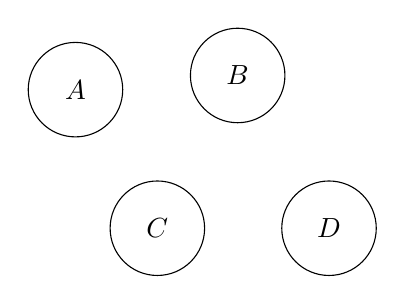
\begin{tikzpicture}[scale=0.2]
\tikzstyle{every node}+=[inner sep=0pt]
\draw [black] (21.3,-20.2) circle (3);
\draw (21.3,-20.2) node {$A$};
\draw [black] (31.6,-19.3) circle (3);
\draw (31.6,-19.3) node {$B$};
\draw [black] (26.5,-29) circle (3);
\draw (26.5,-29) node {$C$};
\draw [black] (37.4,-29) circle (3);
\draw (37.4,-29) node {$D$};
\end{tikzpicture} \\
$ \{A\}, \{B\}, \{C\}, \{D\} \rightarrow $ \texttt{union($A,B$)} $\rightarrow \{A,\hat{B}\}, \{C\}, \{D\}. $
\end{center}

\begin{lstlisting}[mathescape]
kruskal($G=(V,E)$, $w: E \rightarrow R$):
	$T \leftarrow \{\}$
	sort edges so $w(e_1) \leq w(e_2) \leq \ldots \leq w(e_n)$
	for $v \in V$:
		makeset($v$)
	for $i \leftarrow 1$ to $|E|$
		# let $(u_i, v_i) = e_i$
		if find-set($u_i$) != find-set($v_i$):
			$T \leftarrow T \cup \{e_i\}$
	 	if $u_i, v_i$ in different connected components of $T$:
			union($u_i, v_i$)
\end{lstlisting}

\begin{center}
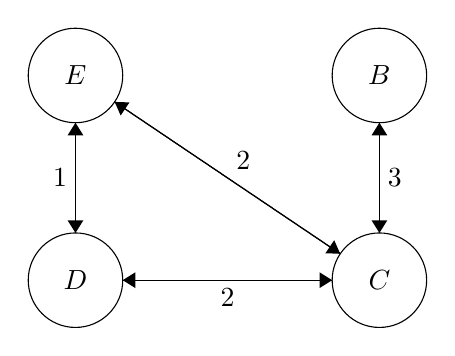
\begin{tikzpicture}[scale=0.2]
\tikzstyle{every node}+=[inner sep=0pt]
\draw [black] (48.5,-18.2) circle (3);
\draw (48.5,-18.2) node {$B$};
\draw [black] (48.5,-31.2) circle (3);
\draw (48.5,-31.2) node {$C$};
\draw [black] (29.2,-18.2) circle (3);
\draw (29.2,-18.2) node {$E$};
\draw [black] (29.2,-31.2) circle (3);
\draw (29.2,-31.2) node {$D$};
\draw [black] (31.69,-19.88) -- (46.01,-29.52);
\fill [black] (46.01,-29.52) -- (45.63,-28.66) -- (45.07,-29.49);
\draw [black] (46.01,-29.52) -- (31.69,-19.88);
\fill [black] (31.69,-19.88) -- (32.07,-20.74) -- (32.63,-19.91);
\draw (39.85,-24.2) node [above] {$2$};
\draw [black] (29.2,-21.2) -- (29.2,-28.2);
\fill [black] (29.2,-28.2) -- (29.7,-27.4) -- (28.7,-27.4);
\draw (28.7,-24.7) node [left] {$1$};
\draw [black] (29.2,-28.2) -- (29.2,-21.2);
\fill [black] (29.2,-21.2) -- (28.7,-22) -- (29.7,-22);
\draw [black] (32.2,-31.2) -- (45.5,-31.2);
\fill [black] (45.5,-31.2) -- (44.7,-30.7) -- (44.7,-31.7);
\draw (38.85,-31.7) node [below] {$2$};
\draw [black] (45.5,-31.2) -- (32.2,-31.2);
\fill [black] (32.2,-31.2) -- (33,-31.7) -- (33,-30.7);
\draw [black] (48.5,-28.2) -- (48.5,-21.2);
\fill [black] (48.5,-21.2) -- (48,-22) -- (49,-22);
\draw (49,-24.7) node [right] {$3$};
\draw [black] (48.5,-21.2) -- (48.5,-28.2);
\fill [black] (48.5,-28.2) -- (49,-27.4) -- (48,-27.4);
\end{tikzpicture} \\

$ \{\hat{C}\}, \{\hat{B}\}, \{\hat{D}\}, \{\hat{E}\} \rightarrow  \{\hat{C}\}, \{\hat{B}\}, \{E,\hat{D}\} \rightarrow \{B\}, \{\hat{D},C,E\} \rightarrow \{\hat{B}, D, C, E\}$
\end{center}


\end{document}
